\subsection{Ground Point Coverage Criterion}
\label{subsec:point_coverage}

One of the fundamental requirements for orbital constellation synthesis in the conducted research is Earth surface specified 
region coverage control. In the absence of additional constraints, surface point is defined as covered by a spacecraft if it simultaneously 
satisfies two conditions: the angular criterion for being within the spacecraft field of view (FOV) and the vector criterion for geometric line-of-sight visibility. 

\paragraph{Angular Ground Point Coverage Criterion}
To satisfy this criterion, the look angle from the spacecraft to the target point $\alpha_v$ must not exceed $\alpha^*$.
The cosine of this angle is defined by the following expression:

\begin{equation}
    \cos{\alpha_{v}}=\frac{-\bf{r_S}\cdot\bf{r_{rel}}}{\left|-\bf{r_S}\right|\times\left|\bf{r_{rel}}\right|}.
\end{equation}

where $\bf{r_S} = (x_S, y_S, z_S)^T$ is the spacecraft position vector, $\bf{r_P} = (x_P, y_P, z_P)^T$ - the ground point position vector, 
and $\bf{r_{rel}} = \bf{r_P} - \bf{r_S}$ is the line-of-sight vector from the spacecraft to the ground point.
Consequently, the relationship for the angle cosines is formulated as follows:
\begin{equation}
    \cos{\alpha_v} \geq \cos{\alpha^*}.
\end{equation}

\paragraph{Vector Ground Point Coverage Criterion}
A line passing through the spacecraft intersects the reference ellipsoid modeling the Earth at two points, except for the case of tangency. 
The point closest to the spacecraft (or the point of tangency) is located on the observable side of the Earth, as the corresponding line segment does not intersect the ellipsoid volume. 
Conversely, the conjugate point is situated on the unobservable side, since the line segment connecting it to the spacecraft passes through the interior of the ellipsoid \ref{fig:point_coverage}.
\begin{figure}[ht]
    \centering
    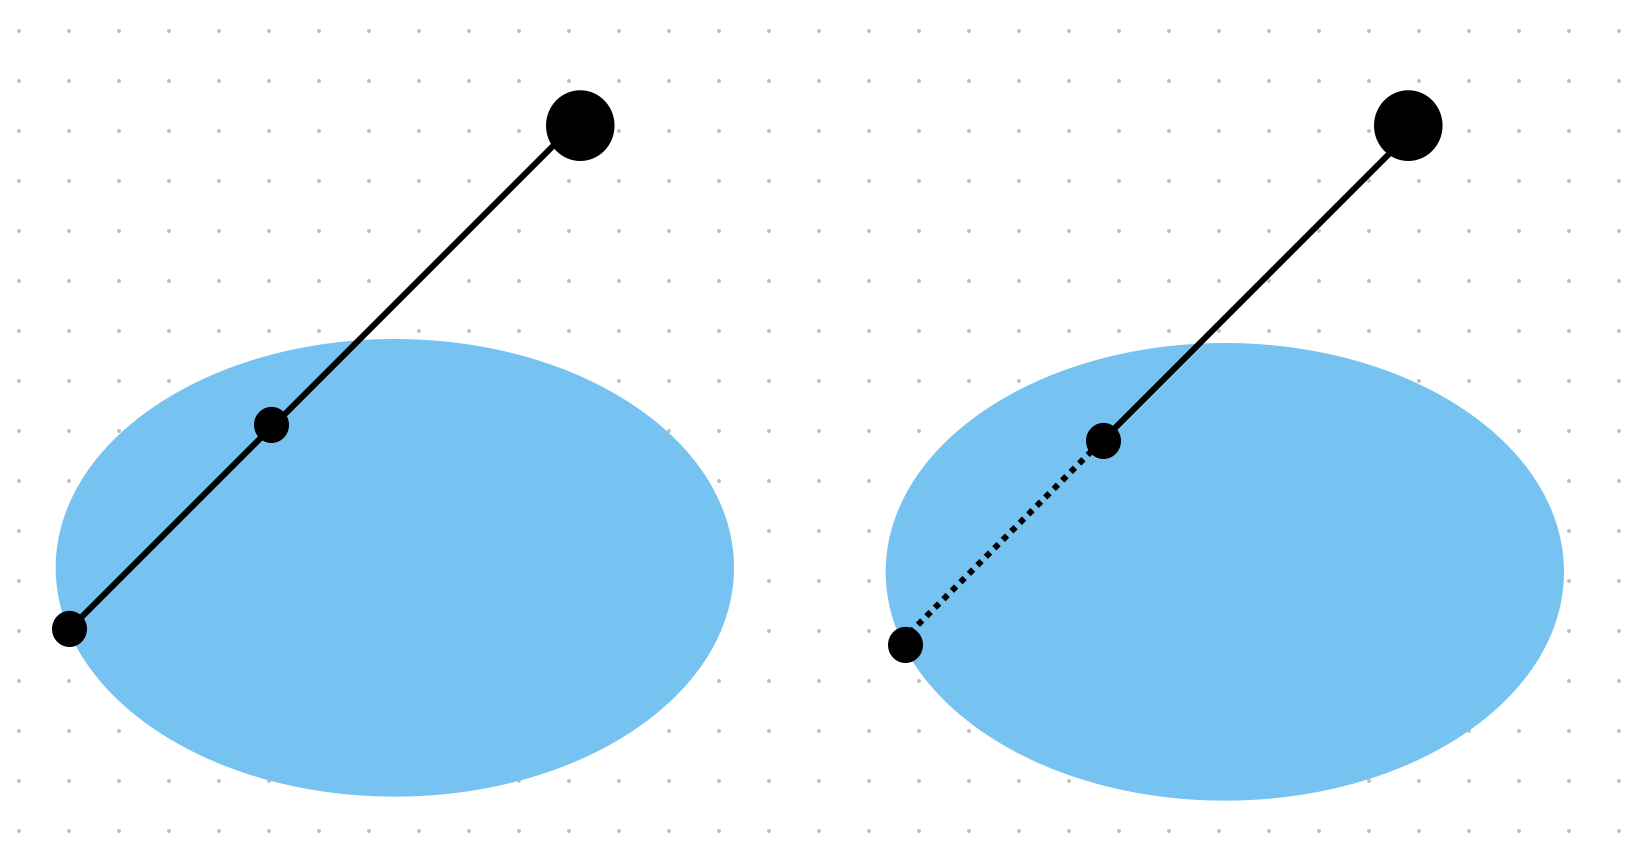
\includegraphics[width=0.75\textwidth]{pictures/point_coverage.png}
    \caption{Ground point coverage}
    \label{fig:point_coverage}
\end{figure}
Surface points satisfying the angular criterion may exist on either side of the Earth, so the vector coverage criterion is introduced to restrict valid points strictly 
to the observable side relative to the spacecraft. Based on this criterion, all surface points are categorized into three cases: 
\begin{itemize}
\item \textbf{The point lies on the observable side of the Earth.} Extending the spacecraft line-of-sight vector $\bf{r_{rel}}$ beyond this point leads to a second intersection with the ellipsoid surface, 
defining the unobservable conjugate point. In this configuration, the vector directed from the observable point to the conjugate point is codirectional with $\bf{r_{rel}} = \bf{r_P} - \bf{r_S}$.
\item \textbf{The point lies on the unobservable side of the Earth.} $\bf{r_{rel}}$ has already intersected the ellipsoid surface on the observable side. The vector directed from this point to its conjugate 
is oppositely directed to $\bf{r_{rel}}$.
\item \textbf{The point is a point of tangency.} Vector analysis is redundant in this case, as the point lacks a conjugate relative to the spacecraft and lies on the observable side of the Earth. 
\end{itemize}
Let the vector equation of the line passing through the spacecraft position and the evaluated ground point be defined as follows:
\begin{equation}\label{eq:line_of_sight}
    \bf{r}=\bf{r}_{P}+\lambda\bf{r}_{rel},
\end{equation}
To determine the intersection points of this line with the ellipsoid, expression \eqref{eq:line_of_sight} is substituted into the ellipsoid equation:
\begin{equation}\label{eq:line_in_ellipsoid}
    \frac{(x_{P}+\lambda x_{rel})^2}{R_E^2} + \frac{(y_{P}+\lambda y_{rel})^2}{R_E^2} + \frac{(z_{P}+\lambda z_{rel})^2}{R_P^2} = 1,
\end{equation}

where $R_E$ denotes the equatorial radius of the reference ellipsoid, and $R_P$ represents its polar radius. 
Expanding the squares and grouping the terms in equation \eqref{eq:line_in_ellipsoid} gives the following equality:
\begin{equation}\label{eq:line_in_ellipsoid_expanded}
    \lambda^2(\frac{x_{rel}^2}{R_E^2}+\frac{y_{rel}^2}{R_E^2}+\frac{z_{rel}^2}{R_P^2})
    +2\lambda (\frac{x_{P}x_{rel}}{R_E^2}+\frac{y_{P}y_{rel}}{R_E^2}+\frac{z_{P}z_{rel}}{R_P^2}) + (\frac{x_{P}^2}{R_E^2}+\frac{y_{P}^2}{R_E^2}+\frac{z_{P}^2}{R_P^2} - 1) = 0,
\end{equation}
which can be expressed in the form:
\begin{equation}\label{eq:line_in_ellipsoid_symbolized}
    \gamma \lambda^2+2\beta\lambda + \kappa = 0.  
\end{equation}
From the solution of quadratic equation \eqref{eq:line_in_ellipsoid_symbolized}:
\begin{equation}\label{eq:line_in_ellipsoid_symbolized_solution}
    \lambda = \frac{-\beta \pm \sqrt{\beta^2-\gamma\kappa}}{\gamma}. 
\end{equation}
Substituting the evaluated point into the line equation \eqref{eq:line_of_sight} yields $\lambda = 0$, which represents the first solution of quadratic equation \eqref{eq:line_in_ellipsoid_symbolized}. 
Thus, quadratic equation \eqref{eq:line_in_ellipsoid_symbolized} either:
\begin{itemize}
\item \textbf{has no real solutions,} which implies that the point does not lie on the Earth surface and is physically unrealizable;
\item \textbf{has a unique solution $\lambda = 0$,} indicating that the point is a point of tangency with the reference ellipsoid;
\item \textbf{has a pair of distinct real solutions $\lambda_1$, $\lambda_2$,} where $\lambda_1 = 0$ corresponds to the evaluated point, and $\lambda_2$ corresponds to its conjugate. 
\end{itemize}
Therefore, whenever equation \eqref{eq:line_in_ellipsoid_symbolized} has a solution, $\lambda_1 = 0$ exists, i.e., substituting it into \eqref{eq:line_in_ellipsoid_symbolized_solution} yields:
\begin{equation}\label{eq:beta_from_ellipsoid}
    \beta = \pm \sqrt{\beta^2 - \gamma\kappa}. 
\end{equation}
From the form of \eqref{eq:line_in_ellipsoid_expanded}, it is obvious that $\gamma>0,\kappa\geq0$. Therefore, taking into account \eqref{eq:line_in_ellipsoid_symbolized_solution} and \eqref{eq:beta_from_ellipsoid}, 
it is shown that $\lambda_2$ satisfying the vector criterion arises only under the condition that $\beta \leq 0$, i.e.:
\begin{equation}\label{eq:vector_coverage_criterion}
    (\frac{x_{P}x_{rel}}{R_E^2}+\frac{y_{P}y_{rel}}{R_E^2}+\frac{z_{P}z_{rel}}{R_P^2}) \leq 0.
\end{equation}

